\section{Results and Discussion}
\label{sec:results}

Empirical results across the four experimental stages defined in Section~\ref{sec:empirics} are presented and analysed in Section~\ref{sec:results}. Subsection~\ref{subsec:res_stage1} examines the Stage~One sample-size learning curves, the effect of reduced-error pruning on natural class distributions, and the deterministic training-accuracy ceiling imposed by conflicting predictor vectors. Subsection~\ref{subsec:res_stage2} analyses the Stage~Two maximum-depth sweeps and the 10,000-row comparison between natural and equal-quota balanced policies. Subsection~\ref{subsec:res_stage3} reports the Stage~Three full-growth-pool tuning pilot. Subsection~\ref{subsec:res_stage4} presents the Stage~Four validation trajectories and the primary evaluation on the reserved generalisation set. Subsection~\ref{subsec:res_perclass} provides a class-level error analysis comparing the four locked approaches. Finally, Subsection~\ref{subsec:res_limits} discusses the methodological limitations of the study.

\subsection{Stage One: Sample-Size Scaling and Feature-Conflict Bounds}
\label{subsec:res_stage1}
Table~\ref{tab:learning_curves} and Figure~\ref{fig:learning_curves} present the Stage~One learning-curve results as the natural-proportion training sample size $n$ at $\lambda = 0$ increased from 2,000 to 50,000 rows across three seeds. Figure~\ref{fig:learning_curves_a} shows validation macro-averaged F1-score $\bar{f}$ and overall accuracy $a$, while Figure~\ref{fig:learning_curves_b} compares observed in-sample training accuracy against the deterministic conflict ceiling.

\begin{table}[!h]
\centering
\caption{Stage One Learning-Curve Results on the Validation Set Across Three Seeds}
\label{tab:learning_curves}
\scriptsize
\setlength{\tabcolsep}{1.3pt}
\begin{tabular}{rlcccc}
\toprule
 & & \multicolumn{3}{c}{\textbf{Validation Set}} & \textbf{Training Set} \\
\cmidrule(lr){3-5} \cmidrule(lr){6-6}
\textbf{Rows ($n$)} & \textbf{Tree} & $\boldsymbol{\bar{f}}$ & $\boldsymbol{a}$ \textbf{(\%)} & $\boldsymbol{\bar{s}}$ \textbf{(\%)} & $\boldsymbol{a}$ \textbf{(\%)} \\
\midrule
 2,000 & Unpruned & $0.4349 \pm 0.0095$ & $74.07 \pm 0.11$ & $43.69 \pm 1.28$ & $99.00 \pm 0.18$ \\
 2,000 & Pruned   & $0.4307 \pm 0.0043$ & $77.23 \pm 0.16$ & $43.15 \pm 0.75$ & $86.65 \pm 0.93$ \\
\midrule
 5,000 & Unpruned & $0.4580 \pm 0.0093$ & $75.50 \pm 0.42$ & $46.14 \pm 0.96$ & $97.99 \pm 0.14$ \\
 5,000 & Pruned   & $0.4585 \pm 0.0068$ & $78.65 \pm 0.34$ & $45.06 \pm 1.23$ & $85.94 \pm 0.22$ \\
\midrule
10,000 & Unpruned & $0.4832 \pm 0.0021$ & $76.75 \pm 0.30$ & $49.00 \pm 0.45$ & $96.63 \pm 0.14$ \\
10,000 & Pruned   & $0.4918 \pm 0.0133$ & $79.69 \pm 0.13$ & $48.38 \pm 1.11$ & $85.58 \pm 0.30$ \\
\midrule
20,000 & Unpruned & $0.5092 \pm 0.0041$ & $77.33 \pm 0.18$ & $51.17 \pm 0.53$ & $95.12 \pm 0.03$ \\
20,000 & Pruned   & $0.5009 \pm 0.0203$ & $80.27 \pm 0.19$ & $49.31 \pm 1.70$ & $85.62 \pm 0.15$ \\
\midrule
50,000 & Unpruned & $0.5506 \pm 0.0118$ & $78.61 \pm 0.20$ & $54.17 \pm 1.31$ & $93.26 \pm 0.02$ \\
50,000 & Pruned   & $0.5362 \pm 0.0061$ & $81.00 \pm 0.21$ & $51.21 \pm 0.90$ & $84.97 \pm 0.22$ \\
\bottomrule
\end{tabular}
\end{table}

\begin{figure*}[!t]
\centering
\subfloat[Validation macro-averaged F1-score and overall accuracy.\label{fig:learning_curves_a}]{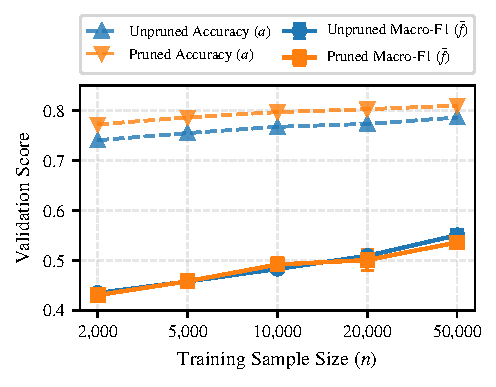
\includegraphics[width=0.47\textwidth]{figures/fig_learning_a.pdf}}\hfill
\subfloat[In-sample training accuracy and deterministic conflict ceiling.\label{fig:learning_curves_b}]{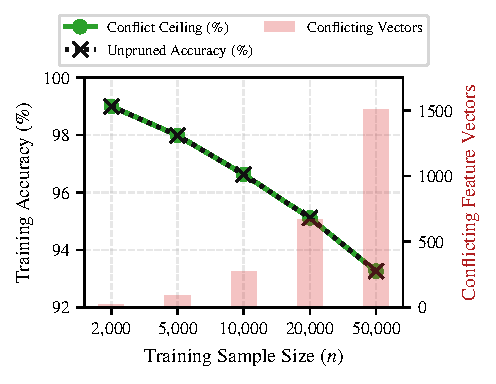
\includegraphics[width=0.47\textwidth]{figures/fig_learning_b.pdf}}
\caption{Stage One sample-size learning curves across $n \in \{2{,}000, 5{,}000, 10{,}000, 20{,}000, 50{,}000\}$ natural-proportion training rows across three seeds.}
\label{fig:learning_curves}
\end{figure*}

Three primary findings emerged from Stage~One:
\begin{enumerate}
    \item \textbf{Sample size governed minority-attack recognition:} As shown in Table~\ref{tab:learning_curves} and Figure~\ref{fig:learning_curves_a}, unpruned validation macro-averaged F1-score increased monotonically with training sample size from $0.4349$ at 2,000 rows to $0.5506$ at 50,000 rows, representing a gain of $0.1157$. Rare-class representation drove the observed gain: a 2,000-row proportional sample contained only one \emph{Worms} observation, six \emph{Shellcode} observations, and 18 \emph{Backdoor} observations, whereas a 50,000-row sample contained 34 \emph{Worms} observations and raised unpruned \emph{Worms} validation F1-score to $0.5450$. Because validation macro-averaged F1-score had not plateaued at 50,000 rows, subsequent final experiments used the entire 123,683-row growth pool.
    \item \textbf{Divergence between accuracy and macro-averaged F1-score under natural pruning:} Reduced-error post-pruning increased validation overall accuracy at every tested sample size by $2.39$ to $3.16$ percentage points, reaching $81.00\%$ at 50,000 rows while reducing the mean leaf count at 50,000 rows from 25,196 to 1,073. However, on naturally skewed samples, post-pruning reduced validation balanced accuracy at every sample size and lowered validation macro-averaged F1-score at 2,000, 20,000, and 50,000 rows, dropping from $0.5506$ to $0.5362$ at 50,000 rows. At 50,000 rows, pruning reduced mean validation recall on \emph{Worms} from $48.8\%$ to $22.6\%$ and reduced \emph{Worms} F1-score from $0.5450$ to $0.3440$. Minimising unweighted error counts on a naturally skewed pruning sample therefore penalised minority-class subtrees when training classes were unbalanced.
    \item \textbf{Deterministic feature-conflict ceiling on training accuracy:} As shown in Table~\ref{tab:learning_curves}, the in-sample training accuracy of unrestricted trees decreased from $99.00\%$ at 2,000 rows to $93.26\%$ at 50,000 rows. Grouping each training sample by all 41 predictor values in Figure~\ref{fig:learning_curves_b} showed that the number of distinct 41-attribute vectors associated with multiple conflicting target labels grew from a mean of $19.0$ at 2,000 rows to $1{,}508.0$ at 50,000 rows out of 35,877 distinct predictor vectors. Because a deterministic classifier assigns a single label to each unique attribute vector, the maximum achievable training accuracy is bounded by predicting the modal label of each identical-vector group. Across all 15 unpruned fits in Table~\ref{tab:learning_curves}, the induced ID3 trees matched the exact deterministic accuracy ceiling in every run, achieving $98.85\%$, $99.20\%$, and $98.95\%$ at 2,000 rows, and $93.284\%$, $93.248\%$, and $93.254\%$ at 50,000 rows.
\end{enumerate}

\subsection{Stage Two: Tree Depth Regularisation and Equal-Quota Balancing at 10,000 Rows}
\label{subsec:res_stage2}
Table~\ref{tab:depth_sweep} and Figure~\ref{fig:depth_curves} report the Stage~Two maximum-depth sweep across $d \in \{0, 1, 2, 4, 8, 12, 20\}$ and unrestricted growth at $n = 10{,}000$ rows under natural ($\lambda = 0$) and equal-quota balanced ($\lambda = 1.0$) policies.

\begin{table}[!h]
\centering
\caption{Stage Two Maximum-Depth Sweep at 10,000 Rows Across Three Seeds}
\label{tab:depth_sweep}
\scriptsize
\setlength{\tabcolsep}{2.5pt}
\begin{tabular}{rcccccc}
\toprule
 & \multicolumn{3}{c}{\textbf{Natural Policy ($\lambda = 0$)}} & \multicolumn{3}{c}{\textbf{Balanced Policy ($\lambda = 1.0$)}} \\
\cmidrule(lr){2-4} \cmidrule(lr){5-7}
\textbf{Depth ($d$)} & \textbf{Train} & \textbf{Validation} & $\boldsymbol{\bar{f}}$ & \textbf{Fit} & \textbf{Validation} & $\boldsymbol{\bar{f}}$ \\
\midrule
0    & 0.6391 & 0.6391 & 0.0530 & 0.9000 & 0.6391 & 0.0530 \\
1    & 0.4343 & 0.4466 & 0.1974 & 0.6651 & 0.7400 & 0.1296 \\
2    & 0.3267 & 0.3525 & 0.2524 & 0.4993 & 0.6348 & 0.2201 \\
4    & 0.2278 & 0.2718 & 0.3191 & 0.2947 & 0.3818 & 0.3825 \\
8    & 0.1434 & \textbf{0.2180} & 0.4627 & 0.1213 & 0.2805 & 0.4761 \\
12   & 0.0838 & 0.2242 & 0.4831 & 0.0613 & 0.2645 & \textbf{0.4841} \\
20   & 0.0427 & 0.2308 & 0.4827 & 0.0335 & 0.2562 & 0.4796 \\
Full & \textbf{0.0337} & 0.2325 & \textbf{0.4832} & \textbf{0.0325} & \textbf{0.2558} & 0.4797 \\
\midrule
Pruned & 0.1442 & \textbf{0.2031} & \textbf{0.4918} & 0.1482 & \textbf{0.2366} & \textbf{0.5021} \\
\bottomrule
\end{tabular}
\end{table}

\begin{figure*}[!t]
\centering
\subfloat[Natural training policy ($\lambda = 0$).\label{fig:depth_curves_a}]{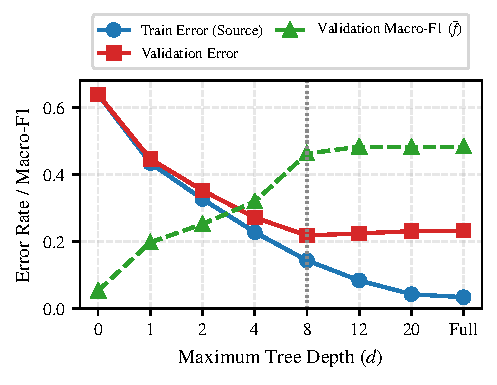
\includegraphics[width=0.47\textwidth]{figures/fig_depth_a.pdf}}\hfill
\subfloat[Equal-quota balanced training policy ($\lambda = 1.0$).\label{fig:depth_curves_b}]{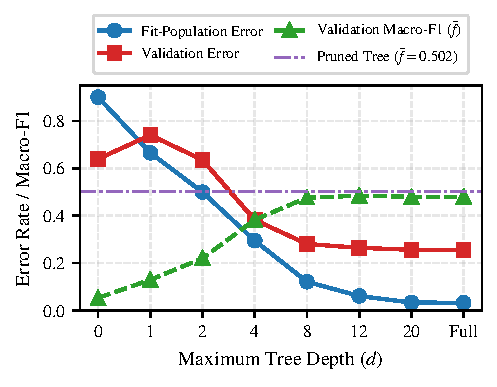
\includegraphics[width=0.47\textwidth]{figures/fig_depth_b.pdf}}
\caption{Stage Two maximum-depth regularisation curves at $n = 10{,}000$ rows across three seeds.}
\label{fig:depth_curves}
\end{figure*}

Under the natural training policy shown in Table~\ref{tab:depth_sweep} and Figure~\ref{fig:depth_curves_a}, source training classification error decreased monotonically from $0.6391$ at $d = 0$ to $0.0337$ at unrestricted depth, whereas validation classification error reached a minimum of $0.2180$ at $d = 8$ and increased to $0.2325$ at unrestricted depth. The divergence between training and validation error beyond $d = 8$ confirmed overfitting in deep unpruned trees under classification error. Validation macro-averaged F1-score $\bar{f}$ increased rapidly up to $\bar{f} = 0.4627$ at $d = 8$ and reached $\bar{f} = 0.4831$ at $d = 12$. Under equal-quota balancing in Figure~\ref{fig:depth_curves_b}, fit-population error decreased from $0.9000$ at $d = 0$ to $0.0325$ at full depth, while validation $\bar{f}$ peaked at $\bar{f} = 0.4841$ for $d = 12$ and declined slightly to $0.4797$ at full depth. Under both policies, bottom-up reduced-error post-pruning outperformed every fixed depth limit, reaching $\bar{f} = 0.4918$ under $\lambda = 0$ and $\bar{f} = 0.5021$ under $\lambda = 1.0$.

Table~\ref{tab:10k_comparison} and Figure~\ref{fig:10k_comparison} compare the standalone trees against 25-member bagging and 25-round depth-three SAMME boosting at the matched 10,000-row budget:
\begin{itemize}
    \item \textbf{Bagging improved over unpruned single trees:} Under natural proportions at $\lambda = 0$, 25-member bagging increased validation $\bar{f}$ relative to the unpruned tree in all three seeds by $+0.0162$, $+0.0208$, and $+0.0075$, raising mean $\bar{f}$ from $0.4832$ to $0.4980$. Under equal-quota balancing at $\lambda = 1.0$, 25-member bagging increased validation $\bar{f}$ over the balanced unpruned tree by $+0.0207$, $+0.0216$, and $+0.0230$, raising mean $\bar{f}$ from $0.4797$ to $0.5015$. Drawing a fresh balanced sample from the 10,000-row source pool for each bagging member also increased distinct source coverage from 4,831--4,846 rows in a single balanced tree to 9,999--10,000 rows across 25 members.
    \item \textbf{Interaction between class balancing and post-pruning:} Applying equal-quota balancing at $\lambda = 1.0$ to an unpruned single tree lowered mean validation $\bar{f}$ from $0.4832$ to $0.4797$, but post-pruning the balanced tree raised validation $\bar{f}$ in every seed to a mean of $0.5021 \pm 0.0017$. The balanced pruned single tree matched 25-member balanced bagging at $\bar{f} = 0.5015 \pm 0.0035$ while requiring a mean fitting time of $49.5\text{ s}$ compared with $1{,}094.9\text{ s}$ for balanced bagging.
    \item \textbf{Accuracy cost of pure equal-quota balancing and underfitting of depth-three boosting:} As shown in Figure~\ref{fig:10k_comparison_b}, equal-quota balancing at $\lambda = 1.0$ increased balanced accuracy $\bar{s}$ across all methods, but reduced overall accuracy $a$ from $79.69\%$ to $76.34\%$ for the pruned tree and from $78.97\%$ to $76.77\%$ for bagging as validation recall on \emph{Normal} traffic dropped from $92.3\%$ to $82.9\%$. Furthermore, although depth-three SAMME boosting improved over a single depth-three tree from $0.2839$ to $0.4383$ under $\lambda = 0$, depth-three base learners lagged behind unrestricted trees and bagging across all settings. Under $\lambda = 1.0$ and $\eta = 0.5$, depth-three boosting achieved a balanced accuracy of $58.34\%$ but an overall accuracy of only $67.34\%$, predicting \emph{Worms} 775 to 1,239 times on a validation set containing 28 true \emph{Worms} records, corresponding to $2.6\%$ precision.
\end{itemize}

\begin{table*}[!t]
\centering
\caption{Stage Two Matched Comparison at 10,000 Source Growth Rows Across Natural ($\lambda=0$) and Equal-Quota ($\lambda=1.0$) Policies Across Three Seeds}
\label{tab:10k_comparison}
\footnotesize
\setlength{\tabcolsep}{2.5pt}
\begin{tabular}{llccccc}
\toprule
\textbf{Method} & \textbf{Policy} & \textbf{Validation $\bar{f}$} & \textbf{Validation $a$ (\%)} & \textbf{Validation $\bar{s}$ (\%)} & \textbf{Train Error (\%)} & \textbf{Fit Time (s)} \\
\midrule
Unpruned Tree                   & Natural ($\lambda=0$)  & $0.4832 \pm 0.0021$ & $76.75 \pm 0.30$ & $49.00 \pm 0.45$ & $3.37 \pm 0.14$  &   $70.3 \pm 4.5$ \\
Pruned Tree                     & Natural ($\lambda=0$)  & $0.4918 \pm 0.0133$ & $\mathbf{79.69 \pm 0.13}$ & $48.38 \pm 1.11$ & $14.42 \pm 0.30$ &   $79.3 \pm 4.9$ \\
Bagging ($t=25$)                & Natural ($\lambda=0$)  & $0.4980 \pm 0.0066$ & $78.97 \pm 0.25$ & $48.81 \pm 0.72$ & $3.56 \pm 0.17$  &  $963.0 \pm 40.3$ \\
Boosting ($t=25, d=3, \eta=0.5$)& Natural ($\lambda=0$)  & $0.4250 \pm 0.0215$ & $76.13 \pm 0.56$ & $41.38 \pm 1.15$ & $19.38 \pm 0.44$ &   $84.6 \pm 6.8$ \\
Boosting ($t=25, d=3, \eta=1.0$)& Natural ($\lambda=0$)  & $0.4383 \pm 0.0097$ & $74.86 \pm 1.47$ & $43.14 \pm 1.58$ & $22.11 \pm 1.80$ &   $54.5 \pm 3.0$ \\
\midrule
Unpruned Tree                   & Balanced ($\lambda=1$) & $0.4797 \pm 0.0036$ & $74.42 \pm 0.37$ & $50.75 \pm 0.12$ & $12.61 \pm 0.60$ &   $43.5 \pm 3.0$ \\
Pruned Tree                     & Balanced ($\lambda=1$) & $\mathbf{0.5021 \pm 0.0017}$ & $76.34 \pm 0.24$ & $53.78 \pm 0.77$ & $17.23 \pm 0.74$ &   $49.5 \pm 3.7$ \\
Bagging ($t=25$)                & Balanced ($\lambda=1$) & $0.5015 \pm 0.0035$ & $76.77 \pm 0.09$ & $53.00 \pm 0.23$ & $6.90 \pm 0.19$  & $1094.9 \pm 15.1$ \\
Boosting ($t=25, d=3, \eta=0.5$)& Balanced ($\lambda=1$) & $0.4261 \pm 0.0099$ & $67.34 \pm 0.39$ & $\mathbf{58.34 \pm 3.12}$ & $28.97 \pm 1.07$ &   $72.1 \pm 2.6$ \\
Boosting ($t=25, d=3, \eta=1.0$)& Balanced ($\lambda=1$) & $0.4305 \pm 0.0184$ & $68.92 \pm 1.52$ & $53.67 \pm 1.82$ & $27.29 \pm 1.11$ &   $47.5 \pm 4.1$ \\
\bottomrule
\end{tabular}
\end{table*}

\begin{figure*}[!t]
\centering
\subfloat[Validation macro-averaged F1-score.\label{fig:10k_comparison_a}]{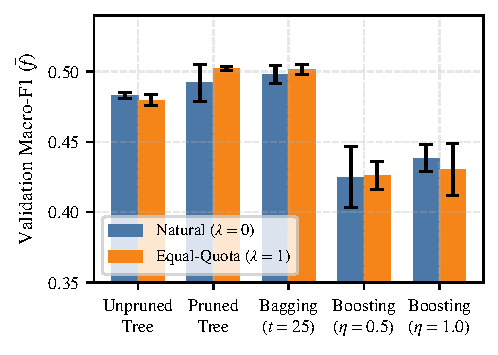
\includegraphics[width=0.47\textwidth]{figures/fig_10k_a.pdf}}\hfill
\subfloat[Validation overall accuracy and balanced accuracy.\label{fig:10k_comparison_b}]{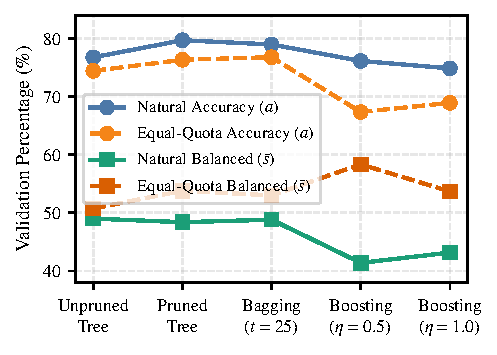
\includegraphics[width=0.47\textwidth]{figures/fig_10k_b.pdf}}
\caption{Stage Two matched 10,000-row comparison across natural ($\lambda = 0$) and equal-quota balanced ($\lambda = 1.0$) policies across three seeds.}
\label{fig:10k_comparison}
\end{figure*}

\subsection{Stage Three: Full-Growth-Pool Hyperparameter Pilot}
\label{subsec:res_stage3}
Stage~Three evaluated the 12 pilot jobs on the full 123,683-row growth pool on seed 42 to compare $\lambda = 0.5$ against $\lambda = 1.0$ and to compare base-tree depths $d \in \{3, 8\}$ and learning rates $\eta \in \{0.5, 1.0\}$ for SAMME boosting. Table~\ref{tab:pilot_results} summarises the resulting validation metrics and wall-clock runtimes.

\begin{table}[!h]
\centering
\caption{Stage Three Full-Growth-Pool Pilot Validation Results on Seed 42}
\label{tab:pilot_results}
\scriptsize
\setlength{\tabcolsep}{1.8pt}
\begin{tabular}{llcccc}
\toprule
\textbf{Configuration} & $\boldsymbol{\lambda}$ & $\boldsymbol{\bar{f}}$ & $\boldsymbol{a}$ \textbf{(\%)} & $\boldsymbol{\bar{s}}$ \textbf{(\%)} & \textbf{Time (s)} \\
\midrule
Unpruned Tree ($t=1$)          & 0.5 & 0.5673 & 77.51 & 57.32 &  360.1 \\
Pruned Tree ($t=1$)            & 0.5 & \textbf{0.6003} & \textbf{80.67} & 61.60 &  400.1 \\
Bagging ($t=5$, Full)          & 0.5 & 0.5852 & 78.94 & 58.77 & 1725.0 \\
Boosting ($t=5, d=3, \eta=0.5$)& 0.5 & 0.3849 & 69.88 & 48.88 &  105.9 \\
Boosting ($t=5, d=3, \eta=1.0$)& 0.5 & 0.4360 & 72.14 & 51.42 &   99.7 \\
Boosting ($t=5, d=8, \eta=0.5$)& 0.5 & 0.5445 & 76.67 & \textbf{61.98} &  646.7 \\
Boosting ($t=5, d=8, \eta=1.0$)& 0.5 & \textbf{0.5587} & 76.58 & 61.76 &  603.6 \\
\midrule
Unpruned Tree ($t=1$)          & 1.0 & 0.5603 & 75.64 & 58.36 &  320.1 \\
Pruned Tree ($t=1$)            & 1.0 & 0.5915 & 78.78 & \textbf{64.43} &  360.5 \\
Bagging ($t=5$, Full)          & 1.0 & 0.5789 & 76.66 & 60.01 & 1567.9 \\
Boosting ($t=5, d=3, \eta=0.5$)& 1.0 & 0.3986 & 62.96 & 55.71 &   98.2 \\
Boosting ($t=5, d=3, \eta=1.0$)& 1.0 & 0.3772 & 60.36 & 54.96 &   95.6 \\
Boosting ($t=5, d=8, \eta=0.5$)& 1.0 & 0.5223 & 73.84 & 63.50 &  746.1 \\
Boosting ($t=5, d=8, \eta=1.0$)& 1.0 & 0.5374 & 73.44 & 62.08 &  701.0 \\
\bottomrule
\end{tabular}
\end{table}

Two findings from Table~\ref{tab:pilot_results} determined the locked settings for Stage~Four:
\begin{enumerate}
    \item \textbf{Superiority of $\lambda = 0.5$ over $\lambda = 1.0$:} Across every model family in Table~\ref{tab:pilot_results}, $\lambda = 0.5$ achieved higher validation macro-averaged F1-score $\bar{f}$ than $\lambda = 1.0$: $0.5673$ versus $0.5603$ for the unpruned tree, $0.6003$ versus $0.5915$ for the pruned tree, $0.5852$ versus $0.5789$ for five-member bagging, and $0.5587$ versus $0.5374$ for depth-eight boosting at $\eta = 1.0$. Simultaneously, $\lambda = 0.5$ preserved $1.87$ to $3.14$ percentage points higher validation overall accuracy $a$ than $\lambda = 1.0$. Under $\lambda = 0.5$, each 123,683-draw sample retained 87,160 distinct source rows from the growth pool compared with 55,872 distinct source rows under $\lambda = 1.0$, preserving substantially broader coverage of \emph{Normal}, \emph{Generic}, and \emph{Exploits} traffic while still allocating at least 6,226 draws to every minority category.
    \item \textbf{Selection of $d = 8$ and $\eta = 1.0$ for boosting:} Increasing the base-tree depth limit from $d = 3$ to $d = 8$ under $\lambda = 0.5$ increased five-round boosting validation $\bar{f}$ from $0.4360$ to $0.5587$ at $\eta = 1.0$ and from $0.3849$ to $0.5445$ at $\eta = 0.5$. Because $d = 8$ with $\eta = 1.0$ achieved the highest validation $\bar{f}$ among the boosting candidates under both $\lambda = 0.5$ and $\lambda = 1.0$, the parameter pair $d = 8$ and $\eta = 1.0$ was selected for the locked primary comparison.
\end{enumerate}

\subsection{Stage Four: Locked Full-Pool Comparison and Ensemble Trajectories}
\label{subsec:res_stage4}

\subsubsection{Validation Trajectories and Structural Complexity}
Table~\ref{tab:final_validation} and Figure~\ref{fig:ensemble_trajectories} report the validation performance, natural-growth scores, and structural complexity of the locked Stage~Four models at $\lambda = 0.5$ across seeds 42 and 43, together with the exploratory extension of bagging to $t = 35$ and $t = 50$ members. All boosting runs fitted all 25 requested members without early termination or learner rejection.

\begin{table*}[!t]
\centering
\caption{Stage Four Full-Growth-Pool Validation Results and Structural Complexity Across Two Seeds}
\label{tab:final_validation}
\footnotesize
\setlength{\tabcolsep}{2.6pt}
\begin{tabular}{lccccccc}
\toprule
\textbf{Method} & \textbf{Members ($t$)} & \textbf{Validation $\bar{f}$} & \textbf{Validation $a$ (\%)} & \textbf{Validation $\bar{s}$ (\%)} & \textbf{Growth $\bar{f}$} & \textbf{Nodes / Leaves / Depth} & \textbf{Size (MB)} \\
\midrule
Unpruned Tree      &  1 & $0.5678 \pm 0.0006$ & $77.39 \pm 0.18$ & $57.55 \pm 0.33$ & $0.7340 \pm 0.0015$ & $40{,}354$ / $29{,}407$ / $50.5$ &  $0.62$ \\
Pruned Tree        &  1 & $\mathbf{0.6087 \pm 0.0119}$ & $\mathbf{80.69 \pm 0.02}$ & $\mathbf{62.97 \pm 1.94}$ & $0.6746 \pm 0.0047$ & $\mathbf{3{,}513}$ / $\mathbf{1{,}861}$ / $42.0$ & $\mathbf{0.08}$ \\
\midrule
Bagging            &  5 & $0.5838 \pm 0.0020$ & $78.79 \pm 0.22$ & $58.61 \pm 0.22$ & $0.7644 \pm 0.0024$ & $2.02 \times 10^5$ total nodes &  $3.39$ \\
Bagging            & 10 & $0.5904 \pm 0.0047$ & $79.22 \pm 0.09$ & $59.34 \pm 0.72$ & $0.7708 \pm 0.0002$ & $4.04 \times 10^5$ total nodes &  $6.86$ \\
Bagging (Locked)   & 25 & $0.6026 \pm 0.0003$ & $79.52 \pm 0.02$ & $61.18 \pm 0.28$ & $\mathbf{0.7735 \pm 0.0000}$ & $1.01 \times 10^6$ total nodes & $17.24$ \\
Bagging (Extended) & 35 & $0.6004 \pm 0.0001$ & $79.57 \pm 0.00$ & $60.95 \pm 0.17$ & $0.7738 \pm 0.0002$ & $1.41 \times 10^6$ total nodes & $24.17$ \\
Bagging (Extended) & 50 & $0.6004 \pm 0.0004$ & $79.66 \pm 0.01$ & $60.86 \pm 0.10$ & $0.7742 \pm 0.0000$ & $2.02 \times 10^6$ total nodes & $34.56$ \\
\midrule
Boosting           &  5 & $0.5537 \pm 0.0071$ & $76.38 \pm 0.28$ & $60.96 \pm 1.13$ & $0.5971 \pm 0.0028$ & $d = 8$ per member &  $0.88$ \\
Boosting           & 10 & $0.5612 \pm 0.0001$ & $75.90 \pm 0.33$ & $60.61 \pm 0.09$ & $0.6105 \pm 0.0028$ & $d = 8$ per member &  $1.75$ \\
Boosting (Locked)  & 25 & $0.5591 \pm 0.0008$ & $76.15 \pm 0.55$ & $58.86 \pm 0.51$ & $0.6290 \pm 0.0026$ & $d = 8$ per member &  $4.38$ \\
\bottomrule
\end{tabular}
\end{table*}

\begin{figure*}[!t]
\centering
\subfloat[Validation macro-averaged F1-score across ensemble size.\label{fig:ensemble_trajectories_a}]{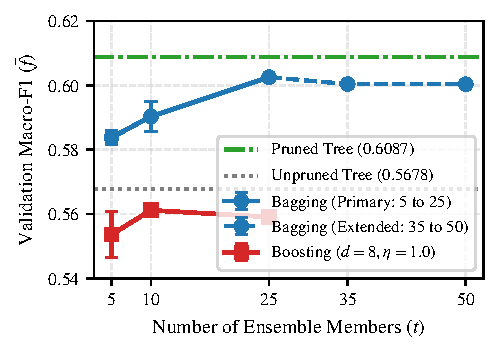
\includegraphics[width=0.47\textwidth]{figures/fig_traj_a.pdf}}\hfill
\subfloat[Validation overall accuracy and balanced accuracy.\label{fig:ensemble_trajectories_b}]{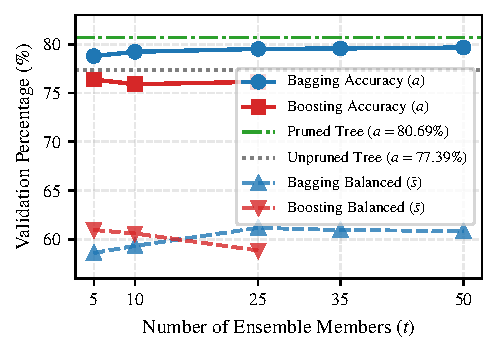
\includegraphics[width=0.47\textwidth]{figures/fig_traj_b.pdf}}
\caption{Stage Four validation trajectories across ensemble size $t$ at full growth-pool scale ($\lambda = 0.5$) across two seeds.}
\label{fig:ensemble_trajectories}
\end{figure*}

Three patterns were observed in Table~\ref{tab:final_validation} and Figure~\ref{fig:ensemble_trajectories}:
\begin{enumerate}
    \item \textbf{Diminishing returns in bagging beyond 25 members:} Increasing the number of bagging members from one unpruned tree at $\bar{f} = 0.5678$ to five, ten, and 25 members steadily increased validation $\bar{f}$ to $0.5838$, $0.5904$, and $0.6026$, while raising validation overall accuracy from $77.39\%$ to $79.52\%$. In the exploratory extension from 25 to 35 and 50 members, validation $\bar{f}$ showed no further gain, remaining at $0.6004$ at both $t = 35$ and $t = 50$ while overall accuracy changed by $+0.14$ percentage points to $79.66\%$.
    \item \textbf{Early plateau of boosting on validation data:} For depth-eight SAMME boosting, natural-growth $\bar{f}$ increased from $0.5971$ at $t = 5$ to $0.6105$ at $t = 10$ and $0.6290$ at $t = 25$. On the validation set, however, $\bar{f}$ peaked at $\bar{f} = 0.5612$ for $t = 10$ and measured $0.5591$ at $t = 25$, while validation balanced accuracy decreased from $60.96\%$ at $t = 5$ to $58.86\%$ at $t = 25$.
    \item \textbf{Structural reduction from reduced-error pruning:} The unpruned full-pool tree averaged 40,354 internal decision nodes, 29,407 leaves, and a depth of $50.5$, occupying $0.62\text{ MB}$ on disk. Reduced-error pruning on the 41,225-row pruning set removed $91.3\%$ of internal nodes and $93.7\%$ of leaves, yielding a mean of 3,513 internal nodes and 1,861 leaves with a disk size of $0.08\text{ MB}$ while increasing validation $\bar{f}$ from $0.5678$ to $0.6087$.
\end{enumerate}

\subsubsection{Primary Generalisation Set Evaluation}
Table~\ref{tab:generalization_summary} reports the primary evaluation of the eight locked models on the reserved 51,531-row generalisation set across seeds 42 and 43.

\begin{table*}[!t]
\centering
\caption{Primary Evaluation on the Reserved Generalisation Set Across Seeds 42 and 43}
\label{tab:generalization_summary}
\footnotesize
\setlength{\tabcolsep}{4.0pt}
\begin{tabular}{lcccccc}
\toprule
\textbf{Approach} & \textbf{Members ($t$)} & \textbf{Seed} & \textbf{Generalisation $\bar{f}$} & \textbf{Overall Accuracy $a$ (\%)} & \textbf{Balanced Accuracy $\bar{s}$ (\%)} & \textbf{Prediction Time (s)} \\
\midrule
Unpruned Tree   &  1 & 42   & 0.5584 & 77.50 & 56.94 & 1.02 \\
Unpruned Tree   &  1 & 43   & 0.5506 & 77.38 & 56.35 & 0.54 \\
\textbf{Unpruned Tree} & \textbf{1} & \textbf{Mean} & $\mathbf{0.5545 \pm 0.0055}$ & $\mathbf{77.44 \pm 0.09}$ & $\mathbf{56.65 \pm 0.41}$ & $\mathbf{0.78 \pm 0.34}$ \\
\midrule
Pruned Tree     &  1 & 42   & 0.6013 & 80.85 & 62.93 & 0.48 \\
Pruned Tree     &  1 & 43   & 0.5973 & 80.61 & 63.12 & 0.48 \\
\textbf{Pruned Tree}   & \textbf{1} & \textbf{Mean} & $\mathbf{0.5993 \pm 0.0028}$ & $\mathbf{80.73 \pm 0.17}$ & $\mathbf{63.02 \pm 0.13}$ & $\mathbf{0.48 \pm 0.00}$ \\
\midrule
Bagging         & 25 & 42   & 0.5752 & 79.65 & 58.63 & 6.65 \\
Bagging         & 25 & 43   & 0.5742 & 79.45 & 58.42 & 6.58 \\
\textbf{Bagging}       & \textbf{25} & \textbf{Mean} & $\mathbf{0.5747 \pm 0.0006}$ & $\mathbf{79.55 \pm 0.14}$ & $\mathbf{58.52 \pm 0.15}$ & $\mathbf{6.61 \pm 0.05}$ \\
\midrule
Boosting ($d=8, \eta=1.0$) & 25 & 42   & 0.5460 & 75.96 & 57.97 & 4.57 \\
Boosting ($d=8, \eta=1.0$) & 25 & 43   & 0.5355 & 76.42 & 56.54 & 5.24 \\
\textbf{Boosting ($d=8, \eta=1.0$)} & \textbf{25} & \textbf{Mean} & $\mathbf{0.5408 \pm 0.0074}$ & $\mathbf{76.19 \pm 0.33}$ & $\mathbf{57.26 \pm 1.01}$ & $\mathbf{4.91 \pm 0.48}$ \\
\bottomrule
\end{tabular}
\end{table*}

The generalisation rankings in Table~\ref{tab:generalization_summary} matched the validation rankings in both seeds:
\begin{enumerate}
    \item \textbf{Pruned single tree:} The pruned tree achieved the highest score on all three primary generalisation metrics with a mean $\bar{f}$ of $0.5993 \pm 0.0028$, an overall accuracy of $80.73\% \pm 0.17\%$, and a balanced accuracy of $63.02\% \pm 0.13\%$. Relative to the unpruned tree, post-pruning improved $\bar{f}$ by $+0.0448$, overall accuracy by $+3.29$ percentage points, and balanced accuracy by $+6.37$ percentage points, while recording the lowest batch prediction time of $0.48\text{ s}$ across the 51,531 rows.
    \item \textbf{Bagging with 25 members:} Bagging ranked second with a mean $\bar{f}$ of $0.5747 \pm 0.0006$, outperforming the unpruned single tree in both seeds by a mean of $+0.0202$ in $\bar{f}$, $+2.11$ percentage points in overall accuracy at $79.55\%$, and $+1.87$ percentage points in balanced accuracy at $58.52\%$. Relative to the pruned single tree, 25-member bagging trailed by $0.0246$ in $\bar{f}$ and $4.50$ percentage points in balanced accuracy while requiring $6.61\text{ s}$ for batch prediction.
    \item \textbf{Unpruned single tree:} The unpruned tree ranked third in $\bar{f}$ at $0.5545 \pm 0.0055$ and third in overall accuracy at $77.44\%$.
    \item \textbf{Boosting with 25 members:} Depth-eight SAMME boosting ranked fourth in $\bar{f}$ at $0.5408 \pm 0.0074$ and fourth in overall accuracy at $76.19\%$, while achieving a higher balanced accuracy at $57.26\%$ than the unpruned single tree at $56.65\%$.
\end{enumerate}

\subsection{Class-Specific Error Analysis and Model Comparison}
\label{subsec:res_perclass}
Table~\ref{tab:generalization_per_class} reports the mean per-class precision $p_j$, recall $s_j$, and F1-score $f_j$ across all ten traffic categories on the generalisation set. Figure~\ref{fig:generalization_per_class} displays the per-class F1-scores, recalls, and precisions, while Figure~\ref{fig:confusion_matrices} presents the row-normalised recall confusion matrices for the pruned tree and 25-member bagging.

\begin{table*}[!t]
\centering
\caption{Per-Class Precision ($p_j$), Recall ($s_j$), and F1-Score ($f_j$) on the Reserved Generalisation Set Across Two Seeds}
\label{tab:generalization_per_class}
\footnotesize
\setlength{\tabcolsep}{4.3pt}
\begin{tabular}{clrrrrrrrrrrrrr}
\toprule
 & & & \multicolumn{3}{c}{\textbf{Unpruned Tree}} & \multicolumn{3}{c}{\textbf{Pruned Tree}} & \multicolumn{3}{c}{\textbf{Bagging ($t=25$)}} & \multicolumn{3}{c}{\textbf{Boosting ($t=25$)}} \\
\cmidrule(lr){4-6} \cmidrule(lr){7-9} \cmidrule(lr){10-12} \cmidrule(lr){13-15}
\textbf{Index ($j$)} & \textbf{Category ($c_j$)} & \textbf{Support} & $p_j$ & $s_j$ & $f_j$ & $p_j$ & $s_j$ & $f_j$ & $p_j$ & $s_j$ & $f_j$ & $p_j$ & $s_j$ & $f_j$ \\
\midrule
1  & Normal         & 18,600 & 0.9057 & 0.9010 & 0.9034 & 0.9098 & 0.9234 & 0.9165 & \textbf{0.9152} & \textbf{0.9349} & \textbf{0.9249} & 0.8998 & 0.8670 & 0.8831 \\
2  & Reconnaissance &  2,797 & 0.8307 & 0.7560 & 0.7916 & \textbf{0.9048} & \textbf{0.7735} & \textbf{0.8340} & 0.8979 & 0.7690 & 0.8285 & 0.7781 & 0.7708 & 0.7744 \\
3  & Backdoor       &    465 & 0.0428 & 0.1817 & 0.0693 & \textbf{0.1027} & 0.1613 & \textbf{0.1252} & 0.0398 & \textbf{0.2183} & 0.0673 & 0.0612 & 0.1806 & 0.0914 \\
4  & DoS            &  3,270 & 0.3212 & 0.3578 & 0.3385 & \textbf{0.3521} & \textbf{0.5740} & \textbf{0.4364} & 0.3387 & 0.3466 & 0.3426 & 0.3086 & 0.3275 & 0.3177 \\
5  & Exploits       &  8,905 & 0.7438 & 0.5970 & 0.6624 & 0.7486 & \textbf{0.6424} & \textbf{0.6915} & \textbf{0.7788} & 0.6218 & \textbf{0.6915} & 0.7013 & 0.6026 & 0.6482 \\
6  & Analysis       &    535 & 0.0541 & 0.1411 & 0.0782 & \textbf{0.1438} & 0.1215 & \textbf{0.1315} & 0.0537 & 0.1215 & 0.0745 & 0.0678 & \textbf{0.1673} & 0.0965 \\
7  & Fuzzers        &  4,849 & 0.6187 & 0.5415 & 0.5775 & 0.6793 & 0.5626 & 0.6154 & \textbf{0.7236} & \textbf{0.5807} & \textbf{0.6444} & 0.5369 & 0.5352 & 0.5360 \\
8  & Worms          &     34 & 0.5417 & 0.5735 & 0.5571 & 0.5351 & \textbf{0.7941} & \textbf{0.6393} & 0.5206 & 0.5588 & 0.5390 & 0.5139 & 0.5147 & 0.5142 \\
9  & Shellcode      &    302 & 0.5388 & 0.6341 & 0.5824 & 0.5138 & 0.7699 & 0.6162 & \textbf{0.5865} & 0.7185 & \textbf{0.6458} & 0.4380 & \textbf{0.7815} & 0.5614 \\
10 & Generic        & 11,774 & 0.9884 & 0.9808 & 0.9846 & \textbf{0.9953} & 0.9798 & 0.9875 & 0.9950 & \textbf{0.9820} & \textbf{0.9885} & 0.9915 & 0.9785 & 0.9850 \\
\midrule
\multicolumn{2}{l}{\textbf{Macro Average}} & \textbf{51,531} & 0.5586 & 0.5665 & 0.5545 & \textbf{0.5885} & \textbf{0.6302} & \textbf{0.5993} & 0.5850 & 0.5852 & 0.5747 & 0.5297 & 0.5726 & 0.5408 \\
\bottomrule
\end{tabular}
\end{table*}

\begin{figure*}[!t]
\centering
\subfloat[Per-class F1-score ($f_j$) across the ten traffic categories.\label{fig:generalization_per_class_a}]{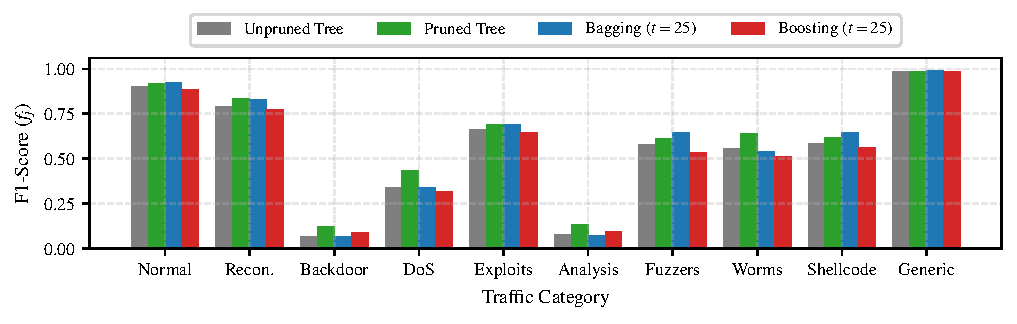
\includegraphics[width=0.92\textwidth]{figures/fig_perclass_a.pdf}}\\
\subfloat[Per-class recall ($s_j$, vertical bars) and precision ($p_j$, black diamonds).\label{fig:generalization_per_class_b}]{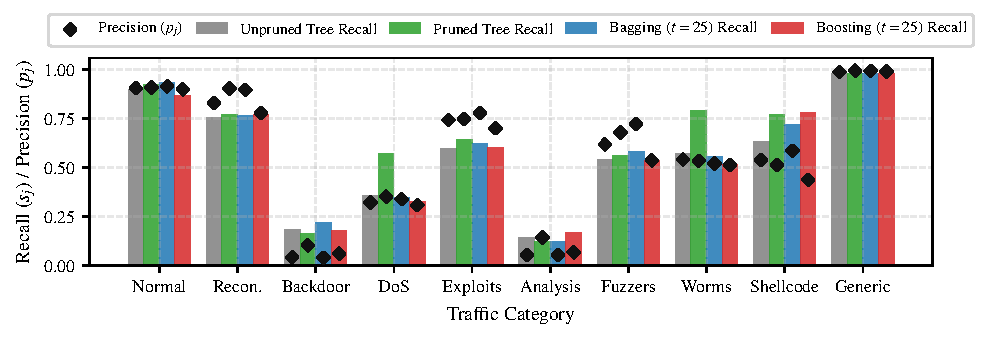
\includegraphics[width=0.92\textwidth]{figures/fig_perclass_b.pdf}}
\caption{Per-class generalisation performance across the ten traffic categories across two seeds.}
\label{fig:generalization_per_class}
\end{figure*}

\begin{figure*}[!t]
\centering
\subfloat[Pruned single decision tree.\label{fig:confusion_matrices_a}]{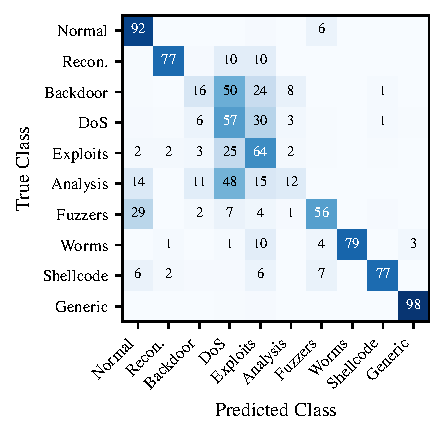
\includegraphics[width=0.46\textwidth]{figures/fig_cm_a.pdf}}\hfill
\subfloat[Bagging with 25 unpruned members.\label{fig:confusion_matrices_b}]{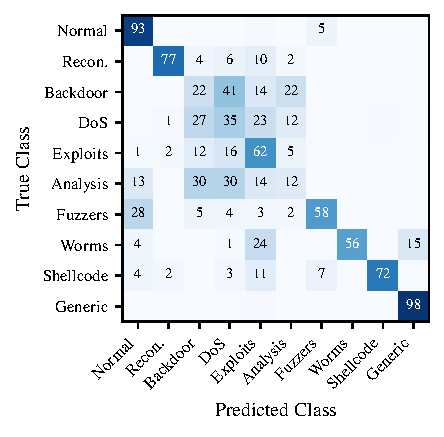
\includegraphics[width=0.46\textwidth]{figures/fig_cm_b.pdf}}
\caption{Row-normalised generalisation confusion matrices showing class recall percentages across seeds 42 and 43.}
\label{fig:confusion_matrices}
\end{figure*}

\subsubsection{Comparison of Pruned Trees and Unpruned Bagging}
Comparing the unpruned standalone tree directly with the corresponding pruned tree in Table~\ref{tab:generalization_per_class} isolates the effect of reduced-error post-pruning on the exact same initial tree fit. Post-pruning increased \emph{Backdoor} precision $p_3$ from $0.0428$ to $0.1027$ and raised $f_3$ from $0.0693$ to $0.1252$. On \emph{Analysis}, post-pruning increased precision $p_6$ from $0.0541$ to $0.1438$ and raised $f_6$ from $0.0782$ to $0.1315$. On \emph{DoS}, post-pruning increased recall $s_4$ from $0.3578$ to $0.5740$ and raised $f_4$ from $0.3385$ to $0.4364$. On \emph{Worms}, post-pruning increased recall $s_8$ from $0.5735$ to $0.7941$ and raised $f_8$ from $0.5571$ to $0.6393$.

When 25 unpruned trees trained under the same $\lambda = 0.5$ balanced distribution were combined via bagging, the ensemble achieved the highest F1-score on four categories in Table~\ref{tab:generalization_per_class}: \emph{Normal} with $f_1 = 0.9249$, \emph{Fuzzers} with $f_7 = 0.6444$, \emph{Shellcode} with $f_9 = 0.6458$, and \emph{Generic} with $f_{10} = 0.9885$, while matching the pruned tree on \emph{Exploits} with $f_5 = 0.6915$. However, on the categories where the $\lambda = 0.5$ training quotas heavily oversampled rare classes that overlap with \emph{DoS} and \emph{Exploits}, unpruned bagging exhibited the same false-positive pattern as the unpruned standalone tree:
\begin{itemize}
    \item As shown in Figure~\ref{fig:confusion_matrices_b}, 25-member bagging misclassified $27\%$ of true \emph{DoS} records and $12\%$ of true \emph{Exploits} records as \emph{Backdoor}, and misclassified an additional $12\%$ of true \emph{DoS} records and $5\%$ of true \emph{Exploits} records as \emph{Analysis}.
    \item As indicated in Table~\ref{tab:generalization_per_class}, the precision of 25-member bagging was $0.0398$ on \emph{Backdoor} and $0.0537$ on \emph{Analysis}, while \emph{DoS} recall was $0.3466$.
    \item In the pruned tree confusion matrix in Figure~\ref{fig:confusion_matrices_a}, false \emph{DoS}-to-\emph{Backdoor} predictions measured only $6\%$ and false \emph{DoS}-to-\emph{Analysis} predictions measured $3\%$, while true \emph{DoS} recall reached $57\%$.
\end{itemize}
The observed contrast between unpruned bagging and the pruned tree is consistent with the difference between averaging unpruned trees trained on an oversampled distribution and post-pruning a balanced tree against a natural-distribution pruning set $P$. While individual internal split paths of the 50 bagging trees were not audited, pruning directly evaluated subtree error counts on the natural class proportions of $P$, collapsing subtrees that generated more false-positive errors on abundant classes than true-positive detections on oversampled classes.

\subsubsection{Multiclass Adaptive Boosting Performance}
Although depth-eight SAMME boosting improved substantially over the depth-three boosting models tested in Stages~Two and~Three, the 25-round generalisation macro-averaged F1-score of boosting reached $\bar{f} = 0.5408$, trailing both 25-member bagging at $0.5747$ and the unpruned single tree at $0.5545$. In Table~\ref{tab:generalization_per_class}, boosting achieved the highest recall on \emph{Analysis} with $s_6 = 0.1673$ and on \emph{Shellcode} with $s_9 = 0.7815$. However, boosting recorded lower recall on \emph{Normal} with $s_1 = 0.8670$ versus $0.9349$ for bagging, lower F1-score on \emph{Fuzzers} with $f_7 = 0.5360$ versus $0.6444$ for bagging, and lower precision on \emph{Shellcode} with $p_9 = 0.4380$ versus $0.5865$ for bagging and on \emph{Reconnaissance} with $p_2 = 0.7781$ versus $0.9048$ for the pruned tree. Lower precision on \emph{Shellcode} and \emph{Reconnaissance} is consistent with the sensitivity of exponential reweighting to label noise and overlapping class boundaries~\cite{Kelleher2020}, documented in Stage~One through the 1,508 conflicting feature vectors at 50,000 rows, although per-instance weight trajectories across the 25 boosting rounds were not separately logged.

\subsection{Methodological Limitations}
\label{subsec:res_limits}
Four methodological constraints govern the interpretation of the experimental findings:
\begin{itemize}
    \item \textbf{Row-based random splitting and repeated feature vectors:} Although the four-way partition was stratified by class, rows were assigned randomly rather than partitioned by capture time window or internet protocol (IP) subnet. Because repeated identical 41-attribute vectors occur in the dataset and were retained to preserve natural flow frequencies during induction and pruning, identical predictor vectors could appear in both the growth and generalisation partitions. Consequently, the reported metrics measure generalisation across held-out rows of the same traffic collection rather than deployment to an unseen network environment.
    \item \textbf{Minority support and oversampling:} The entire 257,673-row dataset contained 174 \emph{Worms} records, with 84 in the growth pool, 28 in the validation pool, and 34 in the generalisation pool. Oversampling 84 records into 6,226 draws increased the weight of \emph{Worms} during split selection, but did not introduce new attack variations. On 34 generalisation instances, a single prediction change altered \emph{Worms} recall $s_8$ by $1/34 \approx 2.94$ percentage points.
    \item \textbf{Unpruned ensemble members and unweighted pruning criterion:} In the locked comparison, reduced-error post-pruning was applied only to the standalone tree, while bagging aggregated unpruned trees. In addition, the pruning criterion in Equation~(\ref{eq:leaf_err}) minimised unweighted classification errors rather than directly maximising macro-averaged F1-score $\bar{f}$.
    \item \textbf{Number of random seeds:} Because full-pool induction on 123,683 rows was computationally intensive, the locked comparison used two random seeds, 42 and 43, evaluated on a single shared generalisation partition. Reported standard deviations therefore describe variation across resampling seeds rather than confidence intervals across independent datasets.
\end{itemize}
